%--------------------------------------------------------------------
% Эта преамбула с комментариями для написания лабораторных работ по
% физике. В еe основе информация из книги С. М. Львовского "Набор и
% верстка в пакете Latex", а также материалы по курсу "Документы и
% презентации в Latex" от ВШЭ https://www.coursera.org/learn/latex. Ну
% и мой опыт (1 год и 16 лабораторных работ + 2 Вопроса по выбору)
% Автор - Баринов Леонид
% Дата - 06.08.2019
%--------------------------------------------------------------------
%--------------------------------------------------------------------
% Для начала необходимо определиться с типом документа. Оптимальный
% (на мой взгляд) вариант - article. Также существуют типы book,
% report, proc и другие. Также в необязательном аргументе можно
% указать тип страницы и размер шрифта. Стандарт по умолчанию - А4 и
% 12 (иногда 10) шрифт. Необязательный аргумент шрифта может принимать
% только 3 параметра - 10, 11, 12 (pt).

\documentclass[a4paper, 12pt]{article}

%--------------------------------------------------------------------
% Чтобы использовать другие размеры шрифта используется пакет
% extsizes. Он позволяет указывать в \documentclass такие размеры - 8,
% 9, 10, 11, 12, 14, 17, 20 (pt). При указании других размеров могут
% возникать различные проблемы.

\usepackage{extsizes}

%--------------------------------------------------------------------
% Необходимо определиться с кодировкой документа. Идеального варианта
% для русского языка не существует - каждый чем-то немного плох. Для
% особо интересующихся - Приложение И в 5 издании книги Львовского. Я
% воспользовался вариантом, предлагаемым на курсе по Latex от ВШЭ.

\usepackage[T2A]{fontenc}
\usepackage[utf8]{inputenc}

%--------------------------------------------------------------------
% Для соблюдения типографских традиций (оказывается такие существуют)
% различных стран создан пакет babel. Самое заметное его действие -
% latex научиться переносить слова того языка, который вы укажите.
% Можно указать несколько языков через запятую. Основной язык
% документа указывается последним.

\usepackage[english,russian]{babel}

%--------------------------------------------------------------------
% Перейдем к заданию полей документа. Есть несколько способов, но
% самый простой из них - это воспользоваться пакетом geometry, который
% позволяет определить все поля документа (начиная с краев листа, что
% важно, так как некоторые другие способы позволяют это сделать только
% косвенно)

\usepackage{geometry}
\geometry{top=25mm}
\geometry{bottom=35mm}
\geometry{left=35mm}
\geometry{right=20mm}

%--------------------------------------------------------------------
% От полей логично перейти к колонтитулам. Тут нам поможет пакет
% fancyhdr. Для него существует 6 колонтитулов - верхний, левый;
% верхний, по центру; верхний, правый и такие же нижние. По умолчанию
% номер страницы находится снизу по центру, а также существует
% линейка, очерчивающие верхний колонтитул. Мне показалось интересным
% сделать колонтитулы схожие с колонтитулами в лабнике. 

\usepackage{fancyhdr}
\pagestyle{fancy}
\renewcommand{\sectionmark}[1]{\markboth{#1}{}} 
% \renewcommand{\headrulewidth}{0mm} % Если необходимо убрать линейку,
% или изменить ее длину
% \lfoot{} % Нижний левый
% \rfoot{} % Нижний правый
% \rhead{} % Верхний правый
% \chead{} % Верхний в центре
\lhead{\thepage} % Номер страницы в левом верхнем углу
\cfoot{} % Оставить нижний колонтитул без цифры

%--------------------------------------------------------------------
% Самое время научиться работать с формулами. А точнее добавить пакеты
% от Американского математического общества, которые позволять
% пользоваться большим количеством математических символов.

\usepackage{amsmath,amsfonts,amssymb,amsthm,mathtools}

%--------------------------------------------------------------------
% Также очень хочется пользоваться русскими буквами в формулах, для
% этого подключаем пакет mathtext, который добавляет окружение
% \text{}. Внутри него можно писать русские буквы в математическом
% режиме.

\usepackage{mathtext}

%--------------------------------------------------------------------
% Большим преимуществом вашего pdf документа будет возможность поиска
% в нем по словам или буквами. (Например, в Ивановнике это
% невозможно)

\usepackage{cmap}

%--------------------------------------------------------------------
% Куда же в физике без картинок и графиков? Давайте исправим
% эту недоработку

\usepackage{graphicx}
\graphicspath{images/} % Необходимо, если рисунки
% находятся в другой папке

%--------------------------------------------------------------------
% graphicx не позволяет вставлять обтекаемые рисунки, но на
% практике они очень нужны. Для этого существует пакет wrapfig

\usepackage{wrapfig}

%--------------------------------------------------------------------
% latex вставляет рисунки по определенному алгоритму. Его,
% конечно, можно менять, но это не настолько просто. Как
% правило, хочется, чтобы картинка располагалась там, где мы это
% указали в коде. Для этого существует несколько пакетов, один из
% них floatrow. Он позволяет для окружения figure указывать
% необязательный аргумент - H (именно большое h), что на latex'овском
% языке означает: вставить картинку здесь и только здесь. (даже если
% облик документа несколько пострадает)

\usepackage{floatrow}

%--------------------------------------------------------------------
% По правилам оформления рисунок всегда должен быть подписан. Для
% этого существует команда \caption{}. Но обычные настройки caption
% меня не совсем устроили. Хотелось сделать подпись меньше
% основного шрифта, а также слово Рис жирным и использовать
% разделитель точку, а не двоеточие. В этом помогает пакет,
% который называется caption (совпадение?)

\usepackage[margin=10pt,font=small,labelfont=bf,labelsep=period]{caption}

%--------------------------------------------------------------------
% Последним важным пунктом остались таблицы. Ведь куда-то нужно
% заносить результаты измерений. На данный момент во время выполнения
% лабораторных работ я заношу результаты в таблицу excel, а потом с
% помощью сайта www.tablesgenerator.com превращаю в таблицу latex и
% дооформляю.

\usepackage{array,tabularx,tabulary,booktabs}

%--------------------------------------------------------------------
% После excel есть ощущения, что везде объединить колонки или строки
% легко. В latex не совсем так. Помогают пакеты multirow, multicol. 

\usepackage{multirow}
\usepackage{multicol}

%--------------------------------------------------------------------
% Иногда могут потребоваться длинные таблицы на несколько страниц.
% Обычные таблицы latex воспринимает как одну букву. И
% становиться понятно, почему возникают проблемы при переносе
% обычной таблицы. (Ведь нельзя же перенести одну букву!). Поэтому
% вместо обычной таблицы нужна длинная таблица.

\usepackage{longtable}

%--------------------------------------------------------------------
% Часто в таблице хочется сделать перенос текста или формулы. Просто
% так это сделать не получиться из-за синтаксиса tabular. Для этого
% каждый раз необходимо создавать новое окружение tabular, что
% утомительно. Поэтому можно ввести команду \specialcell
% (назвать можно по-любому)
    
\newcommand{\specialcell}[2][c]{%
	\begin{tabular}[#1]{@{}c{}}#2\end{tabular}}

%--------------------------------------------------------------------
% Когда в таблице много колонок и строк, кажется, что они находятся
% слишком близко к друг другу. Можно переопределить
% несколько параметров, чтобы выглядело лучше. Это можно сделать либо
% в преамбуле, либо непосредственно в документе. Первое
% переопределение отвечает за интервал между строками, второе за
% интервал между колонками

% \renewcommand{\arraystretch}{1.8} 
% \renewcommand{\tabcolsep}{1cm} 

%--------------------------------------------------------------------
% В русской типографской традиции принято начинать каждый новый абзац
% с красной строки. Даже первый после заголовка (или подзаголовка).
% Чтобы каждый раз не ставить красную строку вручную существует пакет
% indentfirst

\usepackage{indentfirst}

%--------------------------------------------------------------------
% Некоторые модификаторы начертания

\usepackage{soul}
\usepackage{soulutf8}
 
\usepackage{multicol}
\usepackage{mathrsfs}
\usepackage{booktabs}
\begin{document}
\thispagestyle{empty}
\begin{center}
    \textit{Федеральное государственное автономное образовательное\\ учреждение высшего образования }

    \vspace{0.5ex}

        \textbf{«Московский физико-технический институт\\ (национальный исследовательский университет)»}
\end{center}

\vspace{10ex}

\begin{center}
    \vspace{13ex}

    \so{\textbf{Лабораторная работа №_._._}}

    \vspace{1ex}

    по курсу общей физики

    на тему:

    \textbf{\textit{<<>>}}

    \vspace{30ex}

    \begin{flushright}
        \noindent
        \textit{Работу выполнил:}\\  
        \textit{Баринов Леонид \\(группа Б02-827)}
    \end{flushright}
    \vfill
    Долгопрудный \\2019
\newpage
\setcounter{page}{1}
\fancyhead[R]{\nouppercase{\leftmark}}	
\end{center}

\section{Аннотация}
В работе будет проведено измерение
подвижности и концентрации носителей
заряда в металлах.

\section{Теоретические сведения}

Формула проводимости
\begin{equation}
\sigma = e n b
\end{equation}
$b$ -- подвижность, $n$ --
концентрация, $e$ -- элементарный заряд,
показывает что исследование электрической
проводимости проводников позволяет
определить произведение $nb$. Как мы
увидим ниже, исследование эффекта Холла
позволяет находить плотность носителей
$n$, после чего можно найти и их
подвижность $b$. Таким образом,
одновременное исследование электрической
проводимости и эффекта Холла позволяет
экспериментально находить важнейшие
параметры, определяющие состояние
электронов в металлах и полупроводниках.
Эффект Холла позволяет также определить
преобладающий тип проводимости —
электронный или дырочный.

Суть эффекта Холла состоит в следующем.
Пусть через однородную пластину металла
вдоль оси $x$ течёт ток $I$ (рис. 1).

Если эту пластину поместить в магнитное
поле, направленное по оси у, то между
гранями А и Б появляется разность
потенциалов. В самом деле, на электрон,
движущийся со скоростью $\langle
\vec \upsilon \rangle $ в
электромагнитном поле, действует сила
Лоренца:
\begin{equation}
    \vec F_\text{л} = -e\vec E - e
    \langle \vec \upsilon \rangle \times
    \vec B
\end{equation}
где $e$ — абсолютная величина
заряда электрона, $E$ — напряжённость
электрического поля, $B$ — индукция
магнитного поля. В нашем случае сила,
обусловленная вторым слагаемым,
направлена вдоль оси $z$:
\[
    F_B = e|\,\langle \upsilon_x
    \rangle\, |
    B
\]
Здесь $|\,\langle \upsilon_x \rangle\, |$ — абсолютная величина
дрейфовой скорости электронов вдоль оси
$x$, возникающая под действием внешнего
электрического поля.

\begin{wrapfigure}{l}{0.4\linewidth}
    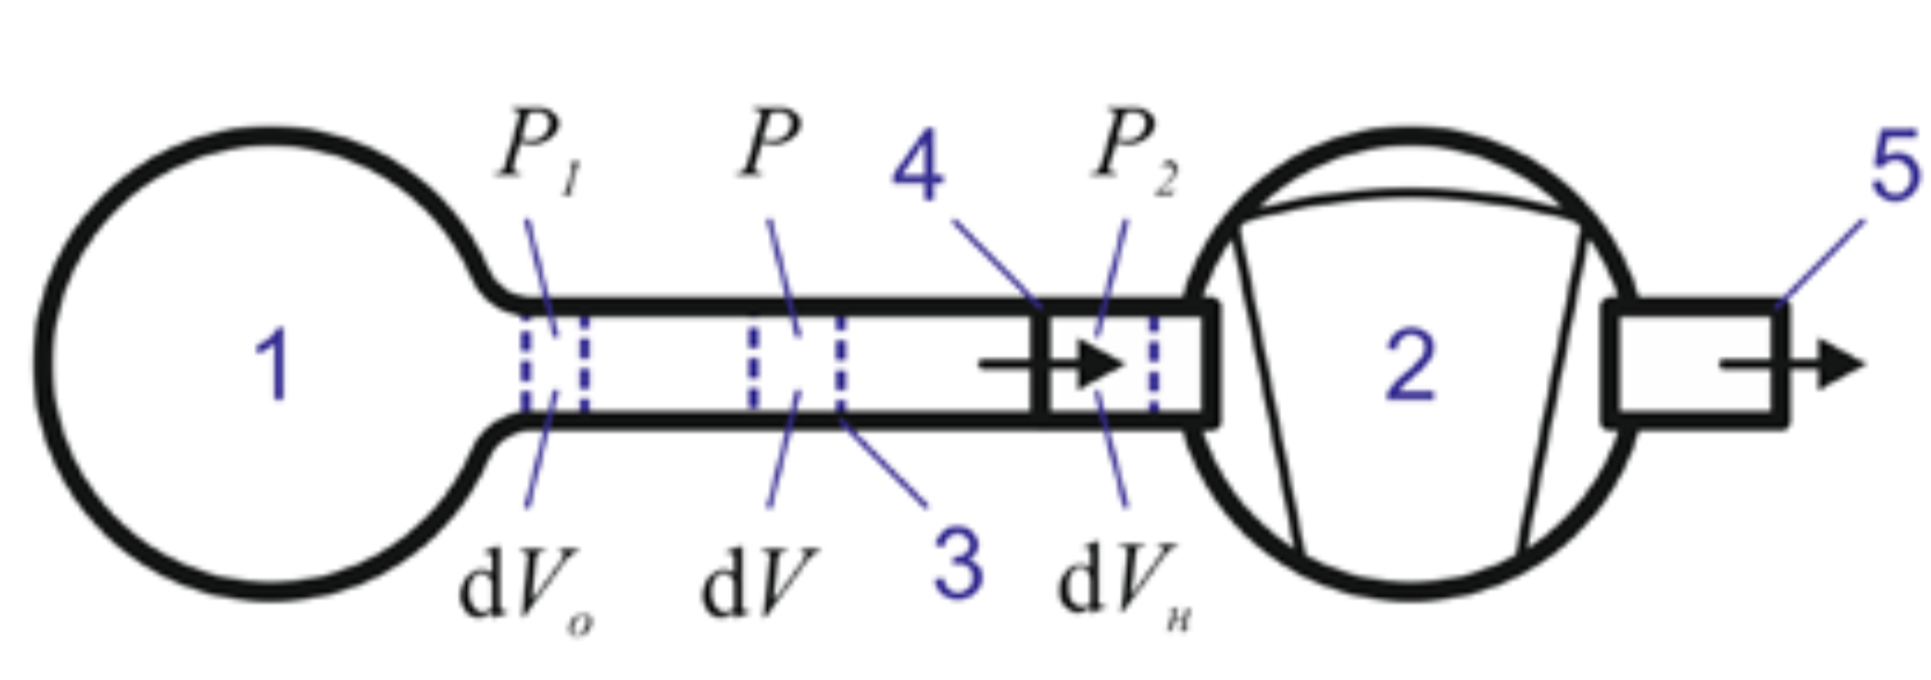
\includegraphics[width=\linewidth]{1}
    \captionsetup{justification=centering}
    \caption{Образец с током в магнитном
    поле}
\end{wrapfigure}

Под действием этой силы электроны
отклоняются к грани Б, заряжая её
отрицательно (для простоты рассматриваем
только один тип носителей). На грани А
накапливаются нескомпенсированные
положительные заряды. Это приводит к
возникновению электрического поля $E_z$,
направленного от А к Б, которое
действует на электроны с силой $F_E =
eE_z$,
направленной против силы $F_B$. В
установившемся режиме сила $F_E$ 
уравновешивает силу $F_B$, И накопление
электрических зарядов на боковых гранях
пластины прекращается. Из условия
равновесия $F_B = F_E$ найдём
\begin{equation}
    E_z = |\, \langle \upsilon_x \rangle
    \, | B
\end{equation}
Поле $E_z$ даёт вклад в общее поле $E$, в
котором движутся электроны. С полем $E_z$ 
связана разность потенциалов
$U_{\text{АБ}}$ между
гранями А и Б:
\begin{equation}
    U_{\text{АБ}} = -E_z l = -
    |\,\langle \upsilon_x \rangle \, | B
    l
\end{equation}
В этом и состоит эффект Холла. Второе
слагаемое в силе Лоренца (2), с
которым связан эффект, часто называют
<<холловским>>.

Замечая, что сила тока
\begin{equation}
    I = ne| \, \langle \upsilon_x
    \rangle \, | l\cdot a,
\end{equation}
и объединяя (3) и (5), найдем ЭДС
Холла:
\begin{equation}
    \mathscr{E}_x = U_\text{АБ} = -
    \frac{IB}{nea} = -R_x \cdot
    \frac{IB}{a}
\end{equation}

Константа $R_x$ называется постоянной
Холла. Как видно из (6):
\[
R_x = \frac{1}{ne}
\]

\section{Оборудование}

\textbf{В работе используются:}
электромагнит с источником питания,
источник постоянного тока,
микровольтметр Ф116/1, амперметры,
милливеберметр, образцы из меди
и цинка.

\subsection*{Экспериментальная установка}
Электрическая схема установки для
измерения ЭДС Холла представлена на рис.
2.

\begin{figure}[H]
    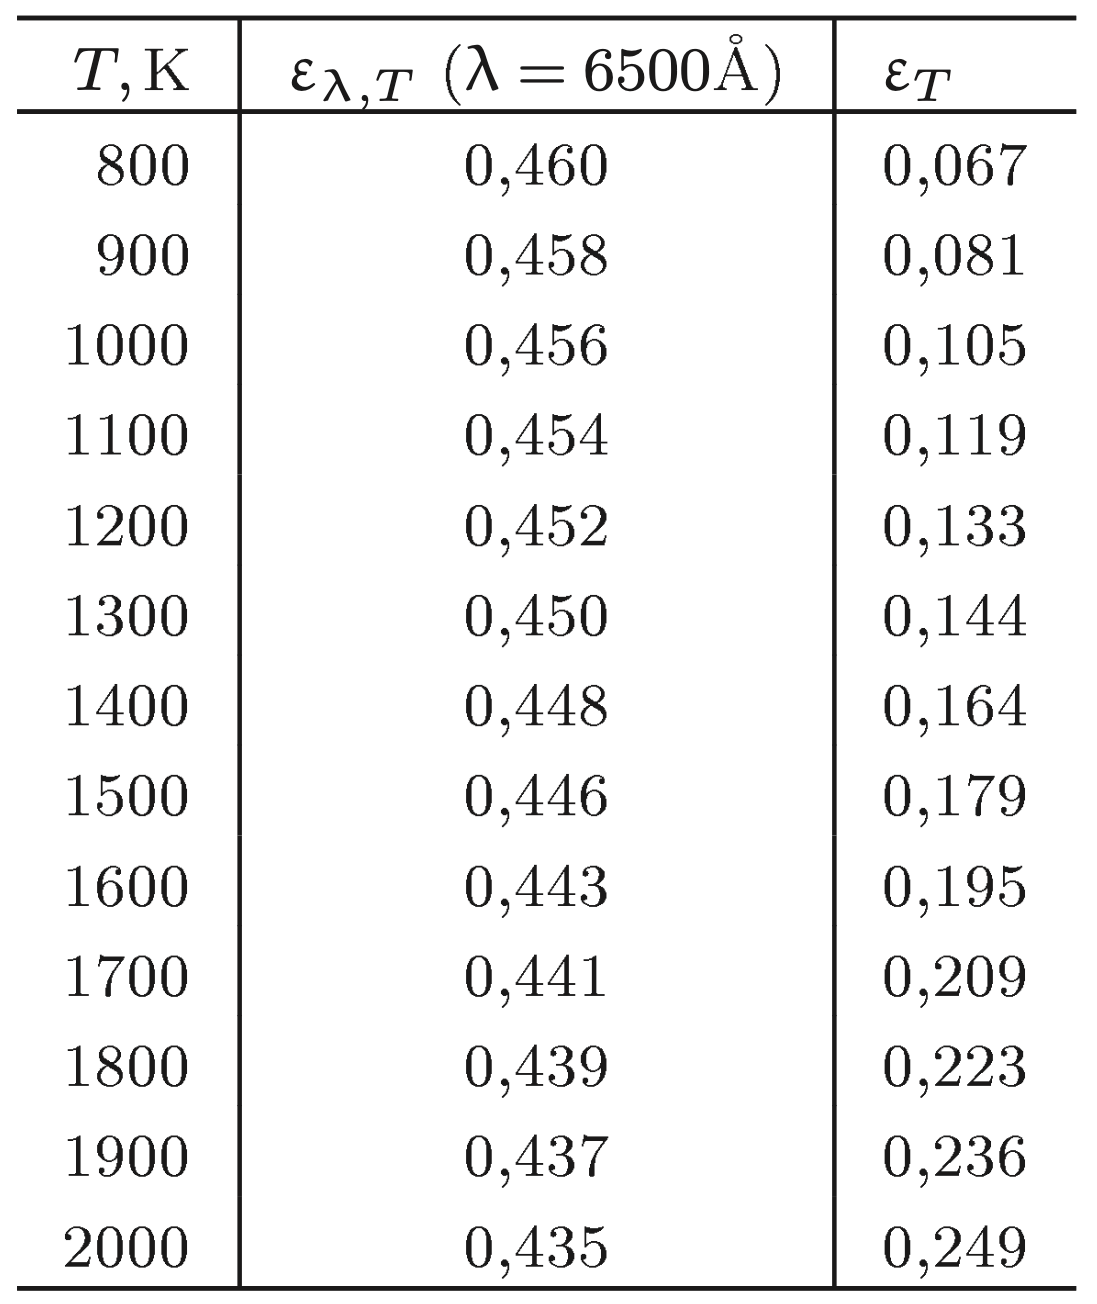
\includegraphics[width=0.725\linewidth]{2} 
    \captionsetup{justification=centering}
    \caption{Схема установки для
    исследования эффекта Холла в
металлах}
\end{figure}

В зазоре электромагнита (рис. 2а)
создаётся постоянное магнитное поле,
величину которого можно менять с помощью
источника питания электромагнита. Разъём
$\text{К}_1$ позволяет менять направление тока в
обмотках электромагнита. Ток питания
электромагнита измеряется амперметром
$\text{А}_1$. Градуировка магнита
проводится с помощью милливеберметра.

Металлические образцы в форме тонких
пластинок, смонтированные в специальных
держателях, подключаются к блоку питания
через разъём (рис. 2б). Ток через
образец регулируется реостатом $R_2$ и
измеряется амперметром $\text{А}_2$.

Для измерений ЭДС Холла используется
микровольтметр Ф116/1, в котором высокая
чувствительность по напряжению
сочетается с малой величиной тока,
потребляемого измерительной схемой:
минимальный предел измерения напряжения
составляет 1,5 мкВ, а потребляемый ток —
всего $10^{-8}$ А.

В образце с током, помещённом в зазор
электромагнита, между контактами 2 и 4
возникает холловская разность
потенциалов, которая измеряется с
помощью микровольтметра, если
переключатель $\text{К}_3$ подключён к точке 2
образца. При подключении $\text{К}_3$ к точке 3
микровольтметр измеряет омическое
падение напряжения $U_{34}$, вызванное
основным током через образец. При
нейтральном положении ключа входная цепь
микровольтметра разомкнута.

Ключ $\text{К}_2$ позволяет менять
полярность напряжения, поступающего на
вход микровольтметра.

Иногда контакты 2 и 4 вследствие
неточности подпайки не лежат на одной
эквипотенциали, и тогда напряжение между
ними связано не только с эффектом Холла,
но и с омическим падением напряжения,
вызванным протеканием основного тока
через образец. Измеряемая разность
потенциалов при одном направлении
магнитного поля равна сумме ЭДС Холла и
омического падения напряжения, а при
другом — их разности. В этом случае ЭДС
Холла $\mathscr{E}_x$ может быть определена как
половина алгебраической разности
показаний вольтметра, полученных для
двух противоположных направлений
магнитного поля в зазоре.

Можно исключить влияние омического
падения напряжения иначе, если при
каждом токе через образец измерять
напряжение $U_0$ между точками 2 и 4 в
отсутствие магнитного поля. При
фиксированном токе через образец это
дополнительное к ЭДС Холла напряжение
остаётся неизменным. От него следует (с
учётом знака) отсчитывать величину ЭДС
Холла:
\begin{equation}
    \mathscr{E}_x = U_{24} \pm U_0
\end{equation}
При таком способе измерения нет
необходимости проводить повторные
измерения с противоположным направлением
магнитного поля.

По знаку $\mathscr{E}_x$ можно определить характер
проводимости — электронный или дырочный.
Для этого необходимо знать направление
тока в образце и направление магнитного
поля.

Измерив ток $I$ в образце и напряжение
$U_{34}$ 
между контактами 3 и 4 в отсутствие
магнитного поля, можно, зная параметры
образца, рассчитать проводимость
материала образца по очевидной формуле:
\begin{equation}
    \sigma = \frac{I L_{34}}{U_{34} a
    l},
\end{equation}
где $L_{34}$ -- расстояние между
контактами 3 и 4, $a$ -- толщина
образца, $l$ -- его ширина.

\section{Результаты измерений и обработка результатов}

Снимем зависимость индукции магнитного
поля от тока через магнит:
\renewcommand{\arraystretch}{1.1} 
\begin{table}[H]
\centering
\begin{tabular}{|c|c|c|c|c|c|c|c|c|}
\hline
$I_\text{М}, \ \text{А}$   & 0  & 0,11 & 0,34 & 0,54 & 0,76
       & 0,95 & 1,03 & 1,27 \\ \hline
$B, \ \text{мТл} $ & 20 & 133  & 414  & 660  & 862
       & 978  & 1012 & 1080 \\ \hline
\end{tabular}
\caption{Зависимость индукции магнитного
поля $B$ от тока через магнит
$I_\text{М}$}
\end{table}

По результатам в таблице 1 построим
график $B=f(I_\text{М})$


\begin{figure}[H]
    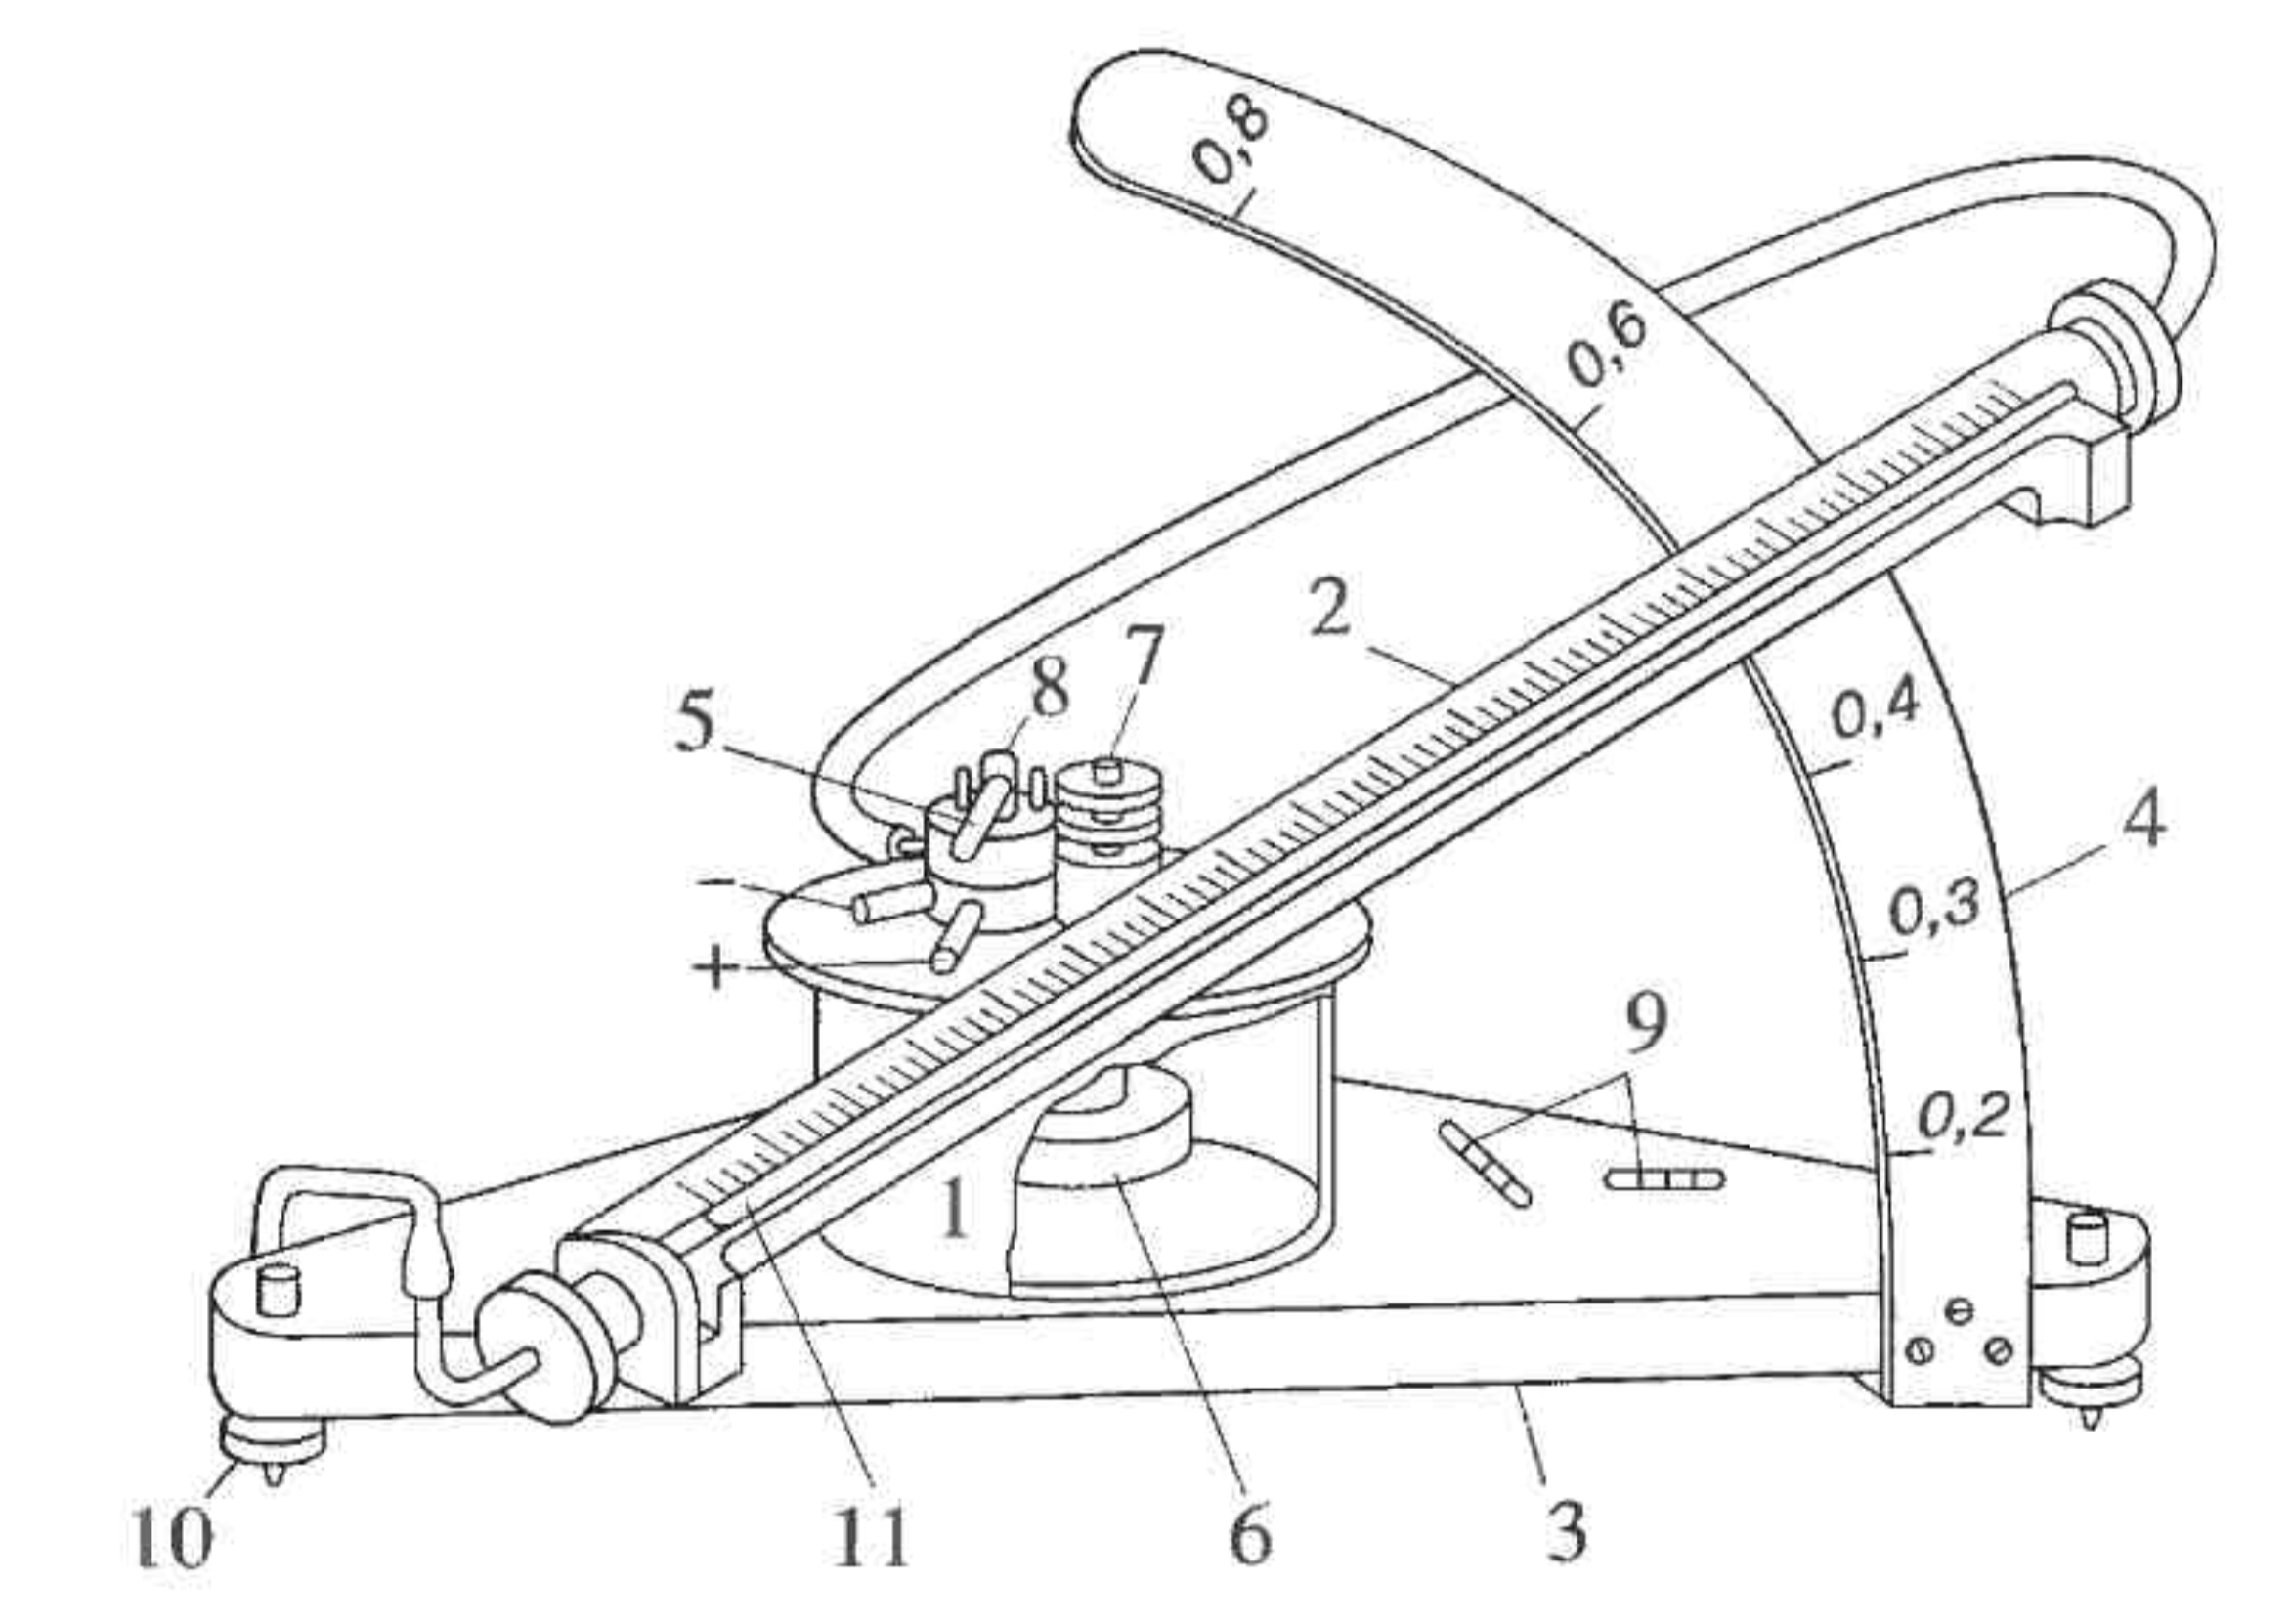
\includegraphics[width=0.9\linewidth]{3} 
    \captionsetup{justification=centering}
    \caption{График зависимости индукции магнитного
поля $B$ от тока через магнит
$I_\text{М}$}
\end{figure}
Рассчитаем ЭДС Холла и построим
семейство характеристик $\mathscr{E} =
f(B)$ при разных значениях тока  $I$
через образец из меди.

%\begin{table}[H]
%\centering
\begin{longtable}{|c|c|c||c|c|c||c|c|c|}
\hline
$I, \ \text{А}$ & $B, \ \text{мТл}$
& $\mathscr{E}, \ \text{мкВ}$    & $I, \ \text{А}$
& $B, \ \text{мТл}$          & $\mathscr{E}, \ \text{мкВ}$    & $I, \ \text{А}$
& $B, \ \text{мТл}$          & $\mathscr{E}, \ \text{мкВ}$    \\ \hline
\endfirsthead
\hline
$I, \ \text{А}$ & $B, \ \text{мТл}$
& $\mathscr{E}, \ \text{мкВ}$    & $I, \ \text{А}$
& $B, \ \text{мТл}$          & $\mathscr{E}, \ \text{мкВ}$    & $I, \ \text{А}$
& $B, \ \text{мТл}$          & $\mathscr{E}, \ \text{мкВ}$    \\ \hline
	\endhead
	\hline
	\endfoot
	\endlastfoot

\multirow{5}{*}{0,2}   & 436,31  & 0,03 & \multirow{12}{*}{0,8} & 178,87  & 0,06 & \multirow{12}{*}{1,01} & 178,87  & 0,09 \\ \cline{2-3} \cline{5-6} \cline{8-9} 
                       & 569,47  & 0,06 &                       & 267,64  & 0,12 &                        & 267,64  & 0,18 \\ \cline{2-3} \cline{5-6} \cline{8-9} 
                       & 640,49  & 0,09 &                       & 356,42  & 0,18 &                        & 356,42  & 0,27 \\ \cline{2-3} \cline{5-6} \cline{8-9} 
                       & 1013,33 & 0,12 &                       & 445,19  & 0,24 &                        & 445,19  & 0,36 \\ \cline{2-3} \cline{5-6} \cline{8-9} 
                       & 1208,63 & 0,12 &                       & 533,96  & 0,33 &                        & 533,96  & 0,45 \\ \cline{1-3} \cline{5-6} \cline{8-9} 
\multirow{8}{*}{0,4}   & 205,50  & 0,06 &                       & 631,61  & 0,42 &                        & 622,73  & 0,54 \\ \cline{2-3} \cline{5-6} \cline{8-9} 
                       & 267,64  & 0,09 &                       & 711,50  & 0,48 &                        & 720,38  & 0,63 \\ \cline{2-3} \cline{5-6} \cline{8-9} 
                       & 383,05  & 0,12 &                       & 800,28  & 0,54 &                        & 800,28  & 0,69 \\ \cline{2-3} \cline{5-6} \cline{8-9} 
                       & 480,70  & 0,18 &                       & 889,05  & 0,57 &                        & 889,05  & 0,75 \\ \cline{2-3} \cline{5-6} \cline{8-9} 
                       & 604,98  & 0,24 &                       & 986,70  & 0,6  &                        & 986,70  & 0,78 \\ \cline{2-3} \cline{5-6} \cline{8-9} 
                       & 782,52  & 0,3  &                       & 1066,59 & 0,63 &                        & 1075,47 & 0,81 \\ \cline{2-3} \cline{5-6} \cline{8-9} 
                       & 1013,33 & 0,33 &                       & 1199,75 & 0,66 &                        & 1190,87 & 0,84 \\ \cline{2-9} 
                       & 1199,75 & 0,33 & \multirow{12}{*}{0,9} & 178,87  & 0,06 & \multirow{12}{*}{1,01} & 178,87  & 0,06 \\ \cline{1-3} \cline{5-6} \cline{8-9} 
\multirow{10}{*}{0,63} & 187,75  & 0,06 &                       & 267,64  & 0,12 &                        & 267,64  & 0,15 \\ \cline{2-3} \cline{5-6} \cline{8-9} 
                       & 276,52  & 0,12 &                       & 356,42  & 0,21 &                        & 356,42  & 0,24 \\ \cline{2-3} \cline{5-6} \cline{8-9} 
                       & 374,17  & 0,18 &                       & 445,19  & 0,3  &                        & 445,19  & 0,36 \\ \cline{2-3} \cline{5-6} \cline{8-9} 
                       & 462,94  & 0,24 &                       & 533,96  & 0,39 &                        & 533,96  & 0,45 \\ \cline{2-3} \cline{5-6} \cline{8-9} 
                       & 560,59  & 0,3  &                       & 640,49  & 0,51 &                        & 631,61  & 0,57 \\ \cline{2-3} \cline{5-6} \cline{8-9} 
                       & 675,99  & 0,36 &                       & 711,50  & 0,54 &                        & 711,50  & 0,63 \\ \cline{2-3} \cline{5-6} \cline{8-9} 
                       & 782,52  & 0,42 &                       & 800,28  & 0,6  &                        & 800,28  & 0,72 \\ \cline{2-3} \cline{5-6} \cline{8-9} 
                       & 889,05  & 0,45 &                       & 906,80  & 0,66 &                        & 889,05  & 0,75 \\ \cline{2-3} \cline{5-6} \cline{8-9} 
                       & 1048,84 & 0,48 &                       & 986,70  & 0,69 &                        & 995,57  & 0,81 \\ \cline{2-3} \cline{5-6} \cline{8-9} 
                       & 1199,75 & 0,51 &                       & 1075,47 & 0,72 &                        & 1066,59 & 0,87 \\ \cline{1-3} \cline{5-6} \cline{8-9} 
\multicolumn{3}{c|}{}                  &
& 1190,87 & 0,75 &
& 1190,87 & 0,87 \\ \cline{4-9}
\captionsetup{justification=centering}
\caption{Зависимость тока $I$ через
образец от магнитной индукции $B$
магнитного поля, в котором находится
образец }
\end{longtable}
%\end{table}

\begin{figure}[H]
    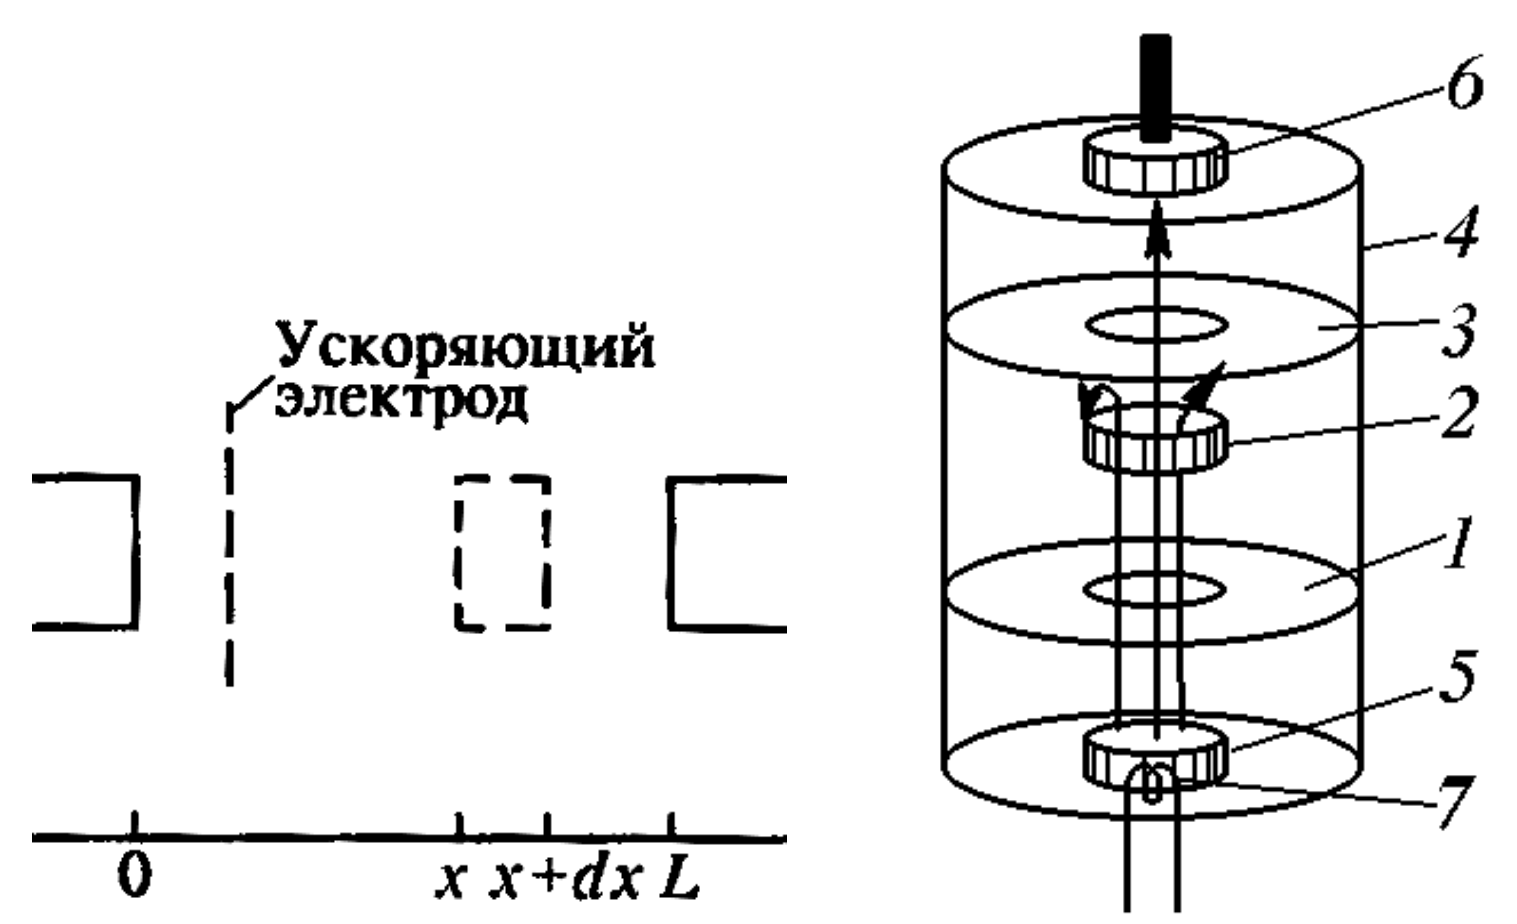
\includegraphics[width=\linewidth]{4} 
    \captionsetup{justification=centering}
    \caption{Семейство характеристик $\mathscr{E} =
    f(B)$ при разных значениях тока  $I$
через образец }
\end{figure}

Определим угловые коэффициенты $k(I) =
\Delta \mathscr{E}/ \Delta B$ полученных
прямых. Построим график $k = f(I)$

\begin{figure}[H]
    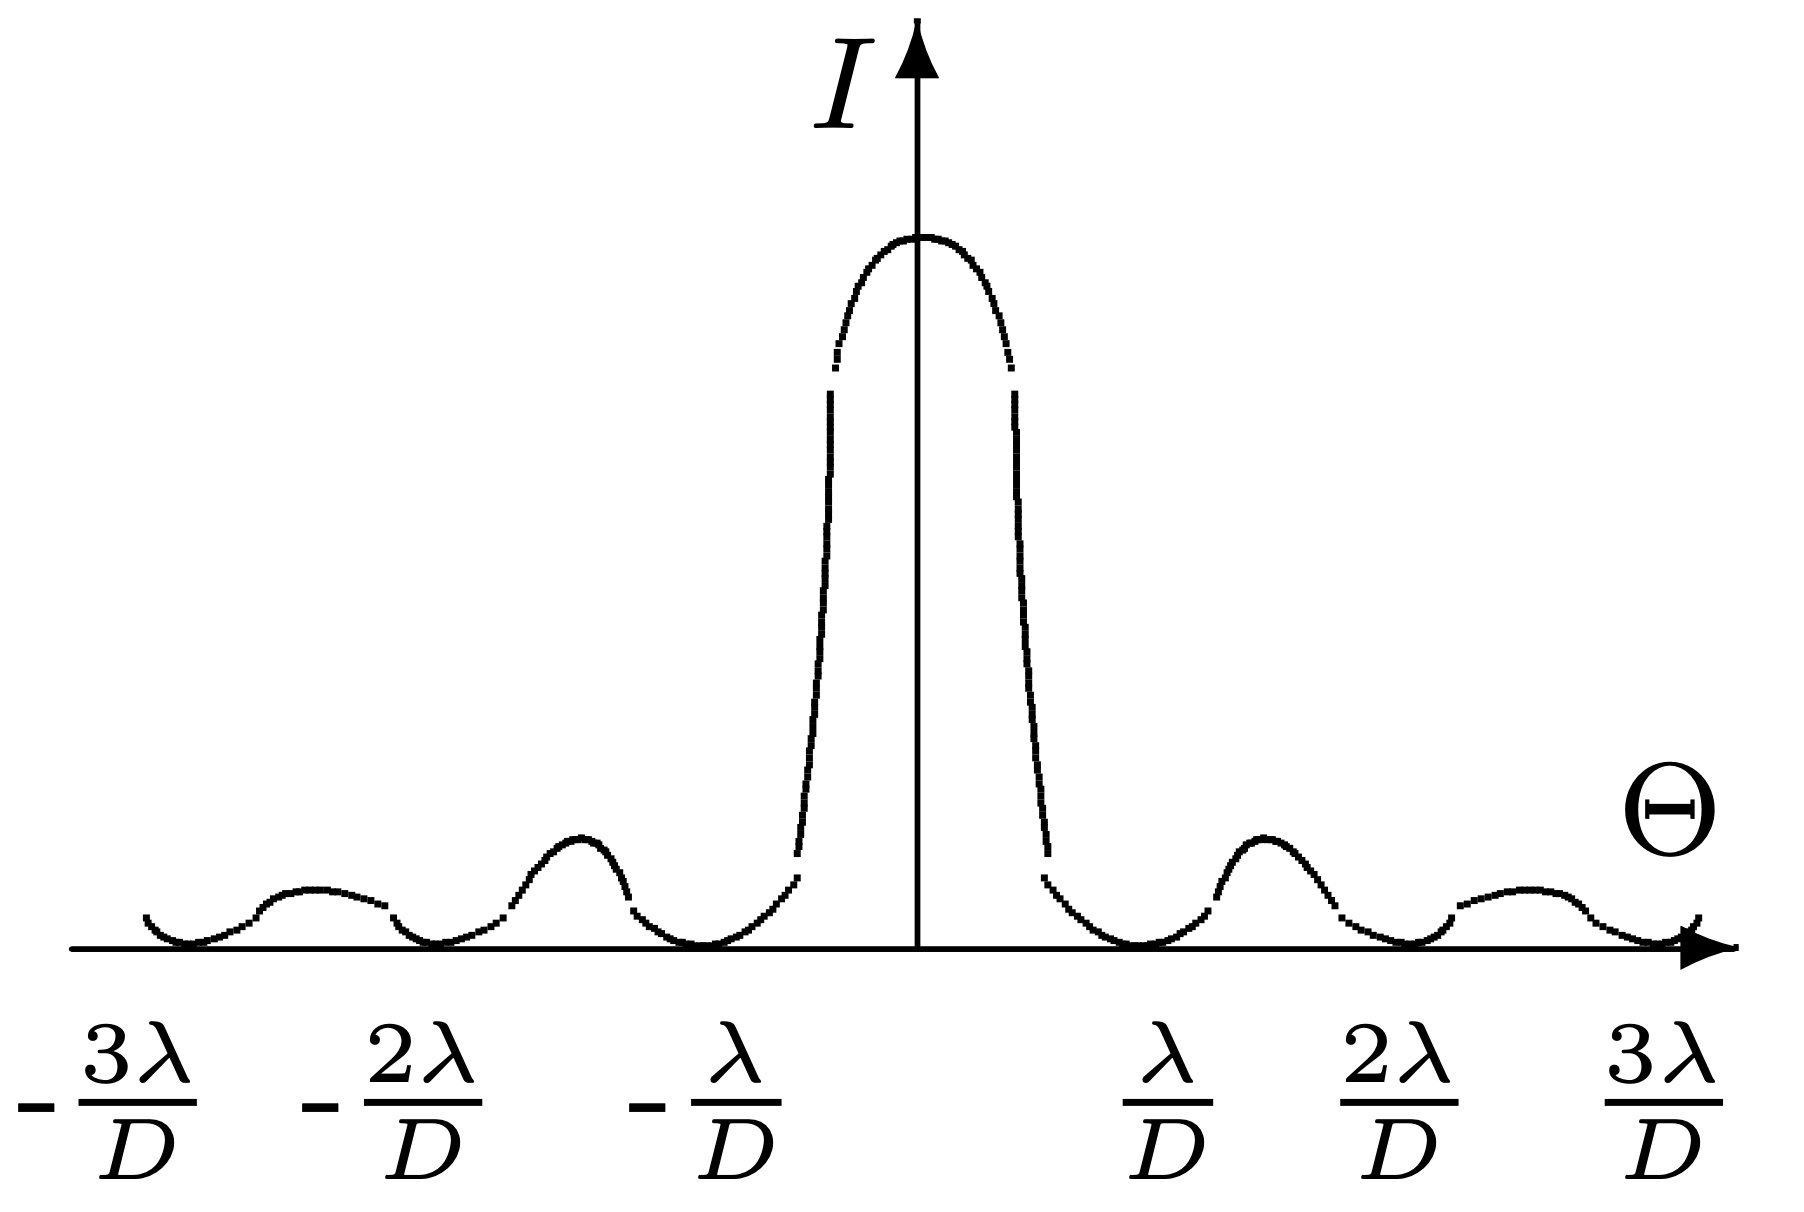
\includegraphics[width=0.85\linewidth]{5} 
    \captionsetup{justification=centering}
    \caption{График зависимости углового
    коэффициента $k = \Delta
\mathscr{E}/ \Delta B$ от тока через
образец $I$}
\end{figure}

Вычислим постоянную Холла по углу
наклона графика на рис. 5. $R_x = -a\cdot t$,
где $t$ -- тангенс угла наклона графика
$k = f(I)$; $a$ = толщина образца из
меди. ($a = 0,05 \ \text{мм}$)
\[
    R_x^\text{медь} = -(0,42\pm 0,08)
    \cdot 10^{-10}\ \text{м}^3/\text{Кл} 
\]

Повторим измерения для образца из цинка.
Построим график зависимости
$\mathscr{E}_x = f(B)$ и по наклону
прямой рассчитаем постоянную Холла $R_x
= -\mathscr{E}_x a/(B I)$ ($a = 0,12\
\text{мм}$, $I = 1\ \text{А}$)

\begin{figure}[H]
    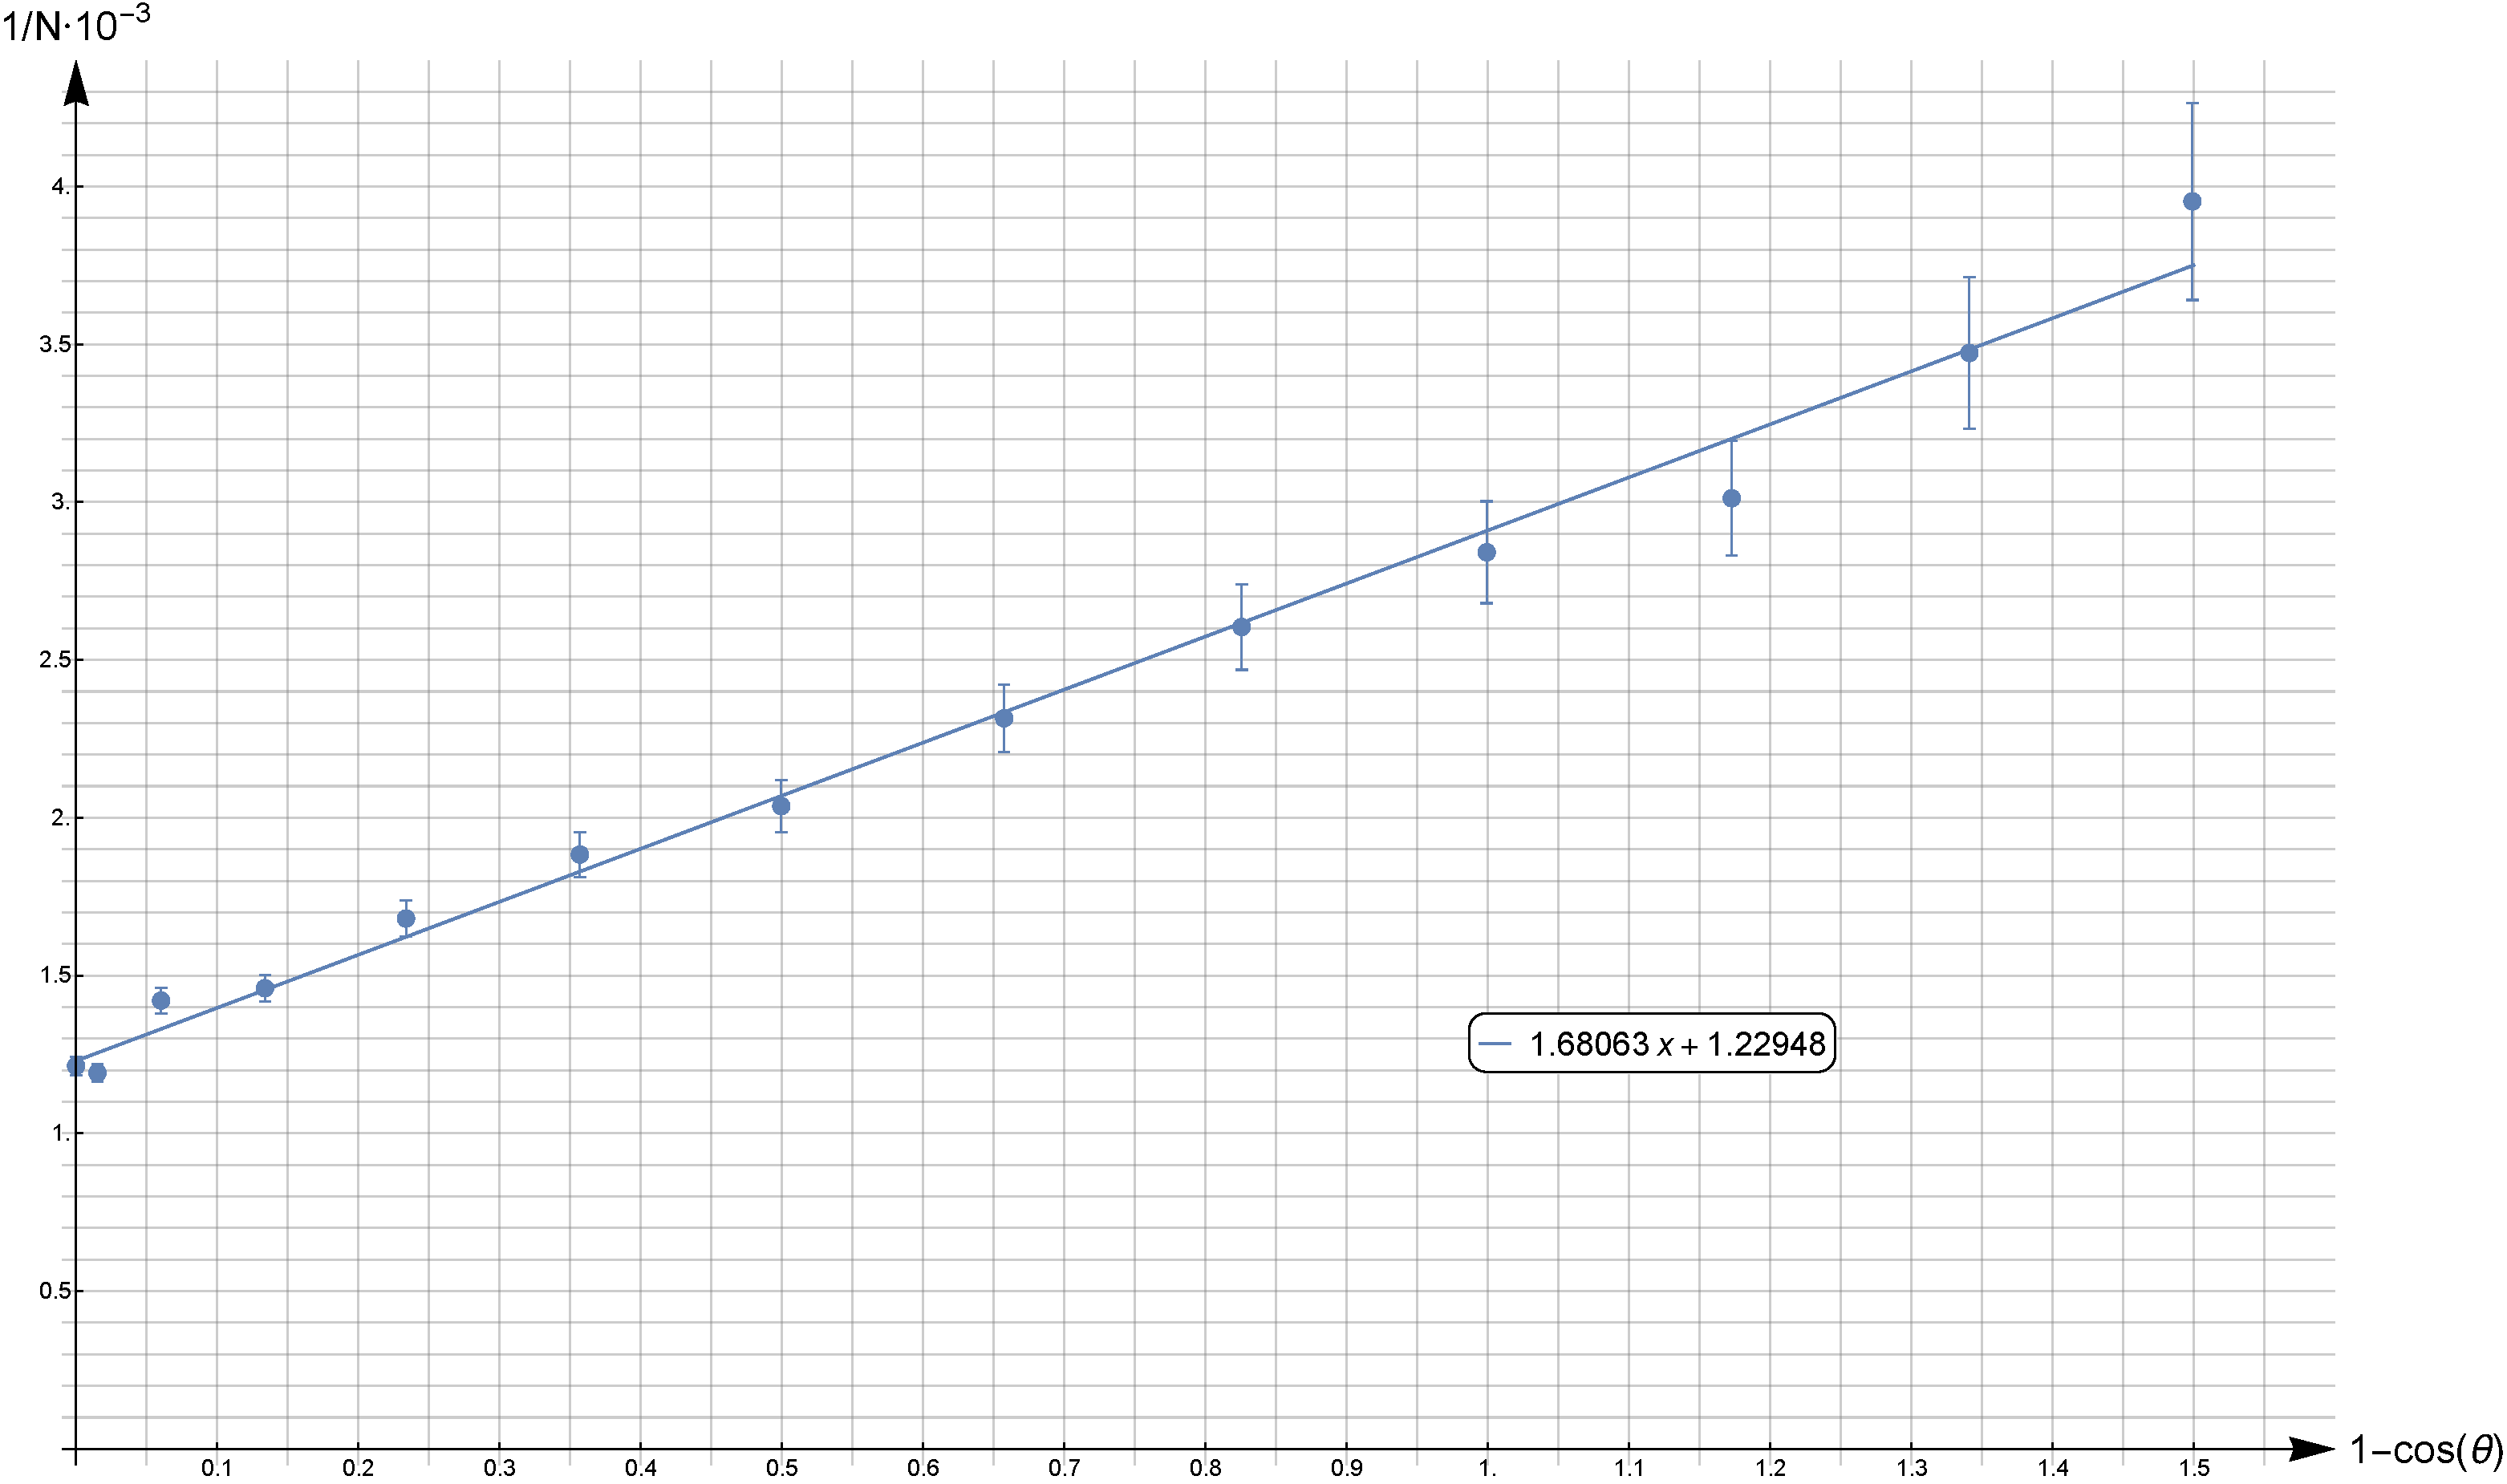
\includegraphics[width=0.85\linewidth]{6} 
    \captionsetup{justification=centering}
    \caption{График зависимости ЭДС
    Холла  $\mathscr{E}$ от магнитной
индукции  $B$ для образца из цинка}
\end{figure}


\[
    R_x^{\text{цинк}} = (1,07 \pm 0,06)
    \cdot 10^{-10} \ \text{м}^3/\text{Кл}
\]

Для определение удельной проводимости
определим значение $U_{34}$ при токе $I
~=~1~\ \text{А}$ 

\begin{equation*}
    \begin{aligned}
        U_{34}^\text{медь} = 240\pm 15 \
        \text{мкВ}\\
        U_{34}^\text{цинк} = 300\pm 15\
        \text{мкВ}
    \end{aligned}
\end{equation*}


Для обоих образцов рассчитаем
концентрацию $n$ носителей тока $n =
1/(R_x e)$. Также вычислим удельную
проводимость $\sigma$ материала образцов
по формуле (8). По результатам
рассчитаем подвижность $b$ носителей
тока.



\begin{table}[H]
    \begin{tabular}{|c|c|c|c|}
        \hline
        Металл & $n, (\text{м}^3)^{-1}$ 
        & $\sigma, \
        (\text{Ом}\cdot\text{м})^{-1}$ &
        $b, \
        \text{см}^2/(\text{B}\cdot\text{с})$ 
        \\ \hline
        Медь & $1,5 \pm 0,3 \cdot
        10^{29}$ & $7,8\pm 0,5 \cdot
        10^{7}$ & $33 \pm 7$ \\ \hline
        Цинк & $6,0 \pm 0,1 \cdot 10^{29}$ & $1,1 \pm
        0,1 \cdot 10^7$ &  $11,4 \pm 1,2$\\ \hline
    \end{tabular}
    \captionsetup{justification=centering}
    \caption{Плотность заряда $n$,
    электропроводность $\sigma$ и
подвижность носителей тока $b$ для
образца из меди и цинка}
\end{table}

\section{Обсуждение результатов и выводы}
\renewcommand{\arraystretch}{1.1} 
\renewcommand{\tabcolsep}{0.1cm} 
Результаты занесены в таблицу.
\begin{table}[H]
    \begin{tabular}{|c|c|c|c|c|c|c|}
        \hline
        Металл & \begin{tabular}{c} $R_x$
            \\ $10^{-10} \text{м}^3
        /\text{Кл}$ \end{tabular} &
        \begin{tabular}{c} Табл. $R_x$, \\
            $10^{-10}\text{м}^3/\text{Кл}$
        \end{tabular}
            & \begin{tabular}{c} Знак\\
            носит. \end{tabular} &
            \begin{tabular}{c} $n$\\
                $10^{29}(\text{м}^3)^{-1}$
            \end{tabular} &
                \begin{tabular}{c}
                    $\sigma$, \\
                    $10^{7}(\text{Ом}\cdot\text{м})^{-1}$
                \end{tabular} &
                \begin{tabular}{c}  $b$,
                    \\
                    $\text{см}^2/(\text{В}\cdot
                \text{с})$
            \end{tabular} \\ \hline
            Медь & $-(0,42 \pm 0,08)$ &
            $-0,53$ &  $-$ & $1,5 \pm
            0,3$ &  $7,8 \pm 0,5$ &
            $33\pm 7$ \\ \hline
            Цинк & $1,07 \pm 0,06$ &
            $1,04$ &  $+$ &  $6,0 \pm
            0,1$ &  $1,1 \pm 0,1$ &
            $11,4\pm 1,2$ \\ \hline
        
    \end{tabular}
    \captionsetup{justification=centering}
    \caption{Постоянная Холла $R_x$, плотность заряда $n$,
    электропроводность $\sigma$ и
подвижность носителей тока $b$ для
образца из меди и цинка}
\end{table}


\end{document}
